\documentclass{beamer}
\usepackage{amsmath}  % Pour les environnements mathématiques
\usetheme{Madrid}
\usepackage{array}  % Pour des options de tableau avancées
\usepackage{booktabs}  % Pour des lignes de tableau plus jolies
\usepackage{multirow}  % Pour les cellules fusionnées
\usepackage{graphicx}  % Pour redimensionner les tableaux et insérer des images
\usepackage{tcolorbox}
\usepackage{fontawesome5}
\usepackage{xcolor}
\usepackage{tikz}

% Définir des couleurs spécifiques pour les sections et sous-sections
\definecolor{sectioncolor}{RGB}{0, 128, 0}      % Vert foncé pour les sections
\definecolor{mycolorlight}{RGB}{155, 204, 155} % Vert clair mélangé avec du blanc (50% de blanc)
\definecolor{titlecolor}{RGB}{0, 128, 64} % Bleu-gris pour les titres de slides
\definecolor{color}{RGB}{34, 139, 34} % Vert clair mélangé avec du blanc (50% de blanc)


\setbeamertemplate{caption}[numbered] %activation de la numérotation des figures et tableau
\setbeamercolor{frametitle}{bg=titlecolor, fg=white}  % Barre des titres des slides en
\setbeamercolor{right footline}{bg=titlecolor, fg=white} % Zone centrale
\setbeamercolor{center footline}{bg=color, fg=white} % Zone droite

% Appliquer la nouvelle couleur aux éléments souhaités
\setbeamercolor{structure}{fg=sectioncolor}  % Change la couleur des titres et des sections


% Définir un bloc avec titre et fond personnalisé
\newtcolorbox[auto counter, number within=section]{myblock}[2][]{%
	colback=sectioncolor!10!white, % Couleur de fond du bloc
	colframe=mycolorlight, % Couleur de bordure du bloc
	colbacktitle=sectioncolor, % Couleur de fond du titre
	coltitle=white, % Couleur du titre
	sharp corners, % Coins du bloc
	boxrule=0.8mm, % Épaisseur de la bordure
	#1 % Options supplémentaires  ,  ,; ,;,;;
}


% Informations sur la présentation
\title{Examen des conditions qui augmentent ou diminuent les différences entre les sexes dans l'engagement dans l'activité physique pendant les cours d'éducation physique, dans le cadre écologique}
\author[Kossi Tonyi Wobubey ABOTSI]{Kossi Tonyi Wobubey ABOTSI \\
	\vspace{0.2cm}
	\textit{Encadré par : Christophe SCHNITZLER}
}
\institute{Stage au Laboratoire E3S}
\date{\today}

% Commande pour définir le nom à afficher
\newcommand{\shortauthorfootline}{Kossi Tonyi Wobubey ABOTSI}
% En-tête personnalisé avec deux zones de couleurs différentes
\setbeamertemplate{headline}{
	\leavevmode%
	\hbox{%
		\begin{beamercolorbox}[wd=.6\paperwidth,ht=2.5ex,dp=1.125ex,center]{section in head/foot}%
			\hspace*{1ex}\insertsectionhead
		\end{beamercolorbox}%
		\begin{beamercolorbox}[wd=.4\paperwidth,ht=2.5ex,dp=1.125ex,center]{subsection in head/foot}%
			\insertsubsectionhead
		\end{beamercolorbox}}%
	\vskip0pt%
}

% Pied de page personnalisé avec trois zones
\setbeamertemplate{footline}{
	\leavevmode%
	\hbox{%
		\begin{beamercolorbox}[wd=.33\paperwidth,ht=2.5ex,dp=1.125ex,left]{author in head/foot}%
			\usebeamerfont{author in head/foot}\shortauthorfootline
		\end{beamercolorbox}%
		\begin{beamercolorbox}[wd=.34\paperwidth,ht=2.5ex,dp=1.125ex,center]{center footline}%
			\usebeamerfont{institute in head/foot}\insertshortinstitute
		\end{beamercolorbox}%
		\begin{beamercolorbox}[wd=.33\paperwidth,ht=2.5ex,dp=1.125ex,right]{right footline}%
			\usebeamerfont{date in head/foot}\insertshortdate{} \hspace*{1.5em}
			\insertframenumber{} / \inserttotalframenumber\hspace*{2ex}
		\end{beamercolorbox}}%
	\vskip0pt%
}

% Définir une nouvelle commande pour afficher le plan avec seulement les sections
\newcommand{\sectiononlytableofcontents}{
	\begin{frame}
		\frametitle{Plan}
		\tableofcontents[hideallsubsections] % Cache les sous-sections
	\end{frame}
}

\begin{document}
	
	% Page de garde avec la barre d'en-tête vide
	{
		\setbeamertemplate{headline}{
			\leavevmode%
			\hbox{%
				\begin{beamercolorbox}[wd=.6\paperwidth,ht=2.5ex,dp=1.125ex,center]{section in head/foot}%
					% Vide pour la page de garde
				\end{beamercolorbox}%
				\begin{beamercolorbox}[wd=.4\paperwidth,ht=2.5ex,dp=1.125ex,center]{subsection in head/foot}%
					% Vide pour la page de garde
			\end{beamercolorbox}}%
			\vskip0pt%
		}
		\begin{frame}
			\titlepage
		\end{frame}
	}
	
	% Slide de Sommaire général
	\sectiononlytableofcontents
	
	% Section 1
	\section{Introduction}
	\begin{frame}
		\tableofcontents[sections={1}]
	\end{frame}
	\subsection{Problématique}
	\begin{frame}
		\frametitle{Problématique} 
		\begin{itemize}
			\item 81 \% des adolescents ne remplissent pas les recommandations de l'OMS en matière d'activité physique
			\vfill
			\pause
			\item Les filles obtiennent en moyenne des résultats inférieurs à ceux des garçons lors des évaluations en éducation physique et sportive (EPS).
			\vfill
			\pause
			\item L'engagement des filles dans l'activité physique à l'adolescence est un enjeu crucial pour leur santé et bien-être, associé aux questions d'équité entre les sexes.
		\end{itemize}
	\end{frame}
	\subsection{Objectifs}
	\begin{frame}
		\frametitle{Objectifs} 
		\begin{itemize}
			\item \textbf{Objectifs générales} \\
			Analyser les différences d'engagement physique entre filles et garçons pendant une leçon d'EPS de 2 heures, en tenant compte de la nature de l'activité (CA), de la catégorie socioculturelle de l'établissement (IPS) et du milieu géographique.
			\vfill
			\pause
			\item \textbf{Objectifs spécifiques} :
				\begin{itemize}
					\item Examen des écarts de niveau d'engagement en EPS entre filles et garçons selon les champs d'apprentissage (CA1, CA2, CA3, CA4).
					\item Examen des écarts de niveau d'engagement en EPS entre filles et garçons selon la catégorie d’IPS du collège (élevé, moyen, faible).
					\item Examen des écarts de niveau d'engagement en EPS entre filles et garçons selon le milieu géographique (urbain, rural).
				\end{itemize}
		\end{itemize}
	\end{frame}

	\section{Méthode}
	\begin{frame}
		\tableofcontents[sections={2}]
	\end{frame}
	\subsection{Présentation des données}
		
		\begin{frame}
			\frametitle{Présentation des données} 
			\begin{itemize}
				\item Les participants âgés de 11 à 15 ans.
				\vfill
				\item MVPA mesuré chez les filles et garçons au cours d'une lecçon d'EPS de 2 heures dans différentes écoles en Alsace et Île-de-France.
			\end{itemize}
			\begin{figure}[H]
				\centering
				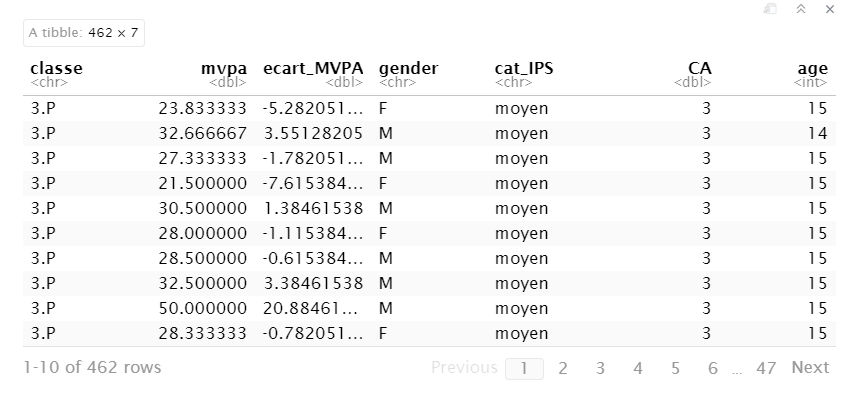
\includegraphics[width=0.95\linewidth]{Extrai_donnée.PNG}
				\caption{Extraits des données}
				\label{fig:image1}
			\end{figure}
		\end{frame}
	\subsection{Modèle}
		\begin{frame}
			\frametitle{Modèles (1/3)} 
			\textcolor{sectioncolor}{\faExclamationTriangle \, Le modèle statistique utilisée est une ANOVA à deux facteurs avec interaction.}
			\pause
			\begin{enumerate}
				\item \textbf{Les facteurs}
				\vfill
				\begin{itemize}
					\item Champs d'apprentissage (CA) à 4 modalités (1, 2, 3 et 4)
					\vfill
					\pause
					\begin{itemize}
						\item \textbf{CA1:} sports de performance (athlétisme, natation, cyclisme, ...)
						\vfill
						\item \textbf{CA2:} sports de plein air et d'aventure (randonnée, alpinisme, surf, ...)
						\vfill
						\item \textbf{CA3:} activité artistique (gymnastique rythmique, patinage artistique, ...)
						\vfill
						\item \textbf{CA4:} sports d'opposition (sport de combat, tennis, ...)
					\end{itemize}
					\pause
					\item Genre à deux modalités (F et M)
				\end{itemize}
				\pause
				\item \textbf{Choix de la variable dépendante :}\\
				Pour analyser les différence d'engagement nous nous basons sur l'écart de MVPA à la moyenne de MVPA de chaque classe.
				\pause
				\begin{itemize}
					\item Cela ajuste les différences de durée d'activité et d'enseignants entre les classes.
				\end{itemize}
				
			\end{enumerate}
		\end{frame}
		
		\begin{frame}
			\frametitle{Modèles (2/3)} 
			Modèle d'ANOVA à deux facteurs (genre et champ d'apprentissage) avec comme variable dépendante l'écart de MVPA par rapport à la moyenne de MVPA de chaque classe.
			
			Le modèle s'écrit :
			\begin{equation}
				Y_{ijk} = \mu + \alpha_i + \beta_j + \gamma_{ij} + \epsilon_{ijk}, \quad i \in \{1,2\}; j\in \{1,2,3,4\},\quad \epsilon_{ijk} \overset{\text{i.i.d}}{\sim} \mathcal{N}(0, \sigma^2) 
			\end{equation}
			où
			\begin{itemize}
				\item $\mu$ est l'effet moyen général,
				\item $\alpha_i$ représente l'effet principal du genre,
				\item $\beta_j$ représente l'effet principal du champ d'apprentissage,
				\item $\gamma_{ij}$ est le terme d'interaction,
				\item $\epsilon_{ijk}$ sont les résidus.
				\item $k$ l'indice de répétition pour le couple $(i,j)$
			\end{itemize}
		\end{frame}
		\begin{frame}
			\frametitle{Modèles (3/3)} 
			\begin{itemize}
				\item Le modèle n'est pas identifiable car pour tout $(1+I+J+IJ)$-uplet $(\mu, \alpha_1, \ldots, \alpha_I, \beta_1, \ldots, \beta_J, \gamma_{11}, \ldots, \gamma_{ij}, \ldots, \gamma_{IJ})^\top$ et pour tout $a \in \mathbb{R}$, le $(1+I+J+IJ)$-uplet $(\mu-a, \alpha_1+\frac{a}{3}, \ldots, \alpha_I+\frac{a}{3}, \beta_1+\frac{a}{3}, \ldots, \beta_J+\frac{a}{3}, \gamma_{11}+\frac{a}{3}, \ldots, \gamma_{ij}+\frac{a}{3}, \ldots, \gamma_{IJ}+\frac{a}{3})^\top$ correspond au même modèle.
				\vfill
				\item On utilise la contrainte de somme :
				\begin{equation*}
					\sum_{i} \alpha_i = 0; \quad \sum_{j} \beta_j = 0; \quad \forall i, \quad \sum_{j} \gamma_{ij} = 0; \quad \forall j, \quad \sum_{i} \gamma_{ij} = 0
				\end{equation*}
			\end{itemize}
		\end{frame}
		
		
	\subsection{Validation des hypothèses}
		\begin{frame}
			\frametitle{Condition d'application du modèle} 
			\begin{itemize}
				\item \textcolor{sectioncolor}{Indépendance des observations (ou des résidus).}
				\vfill
				\item \textcolor{sectioncolor}{Égalité des variances des résidus du modèle (homoscédasticité).}
				\vfill
				\item \textcolor{sectioncolor}{Normalité des résidus du modèle.}
			\end{itemize}
		\end{frame}
		
		\begin{frame}{Indépendance des observations}
			L'hypothèse d'indépendance des observations est vérifiée. La liaison potentielle due à l'appartenance à une même classe ou école est éliminée du à l'utilistation de l'écart de MVPA à la moyenne du MVPA pour chaque classe.
		\end{frame}
		
		\begin{frame}{Égalité des variances des résidus du modèle}
			\begin{figure}[H]
				\centering
				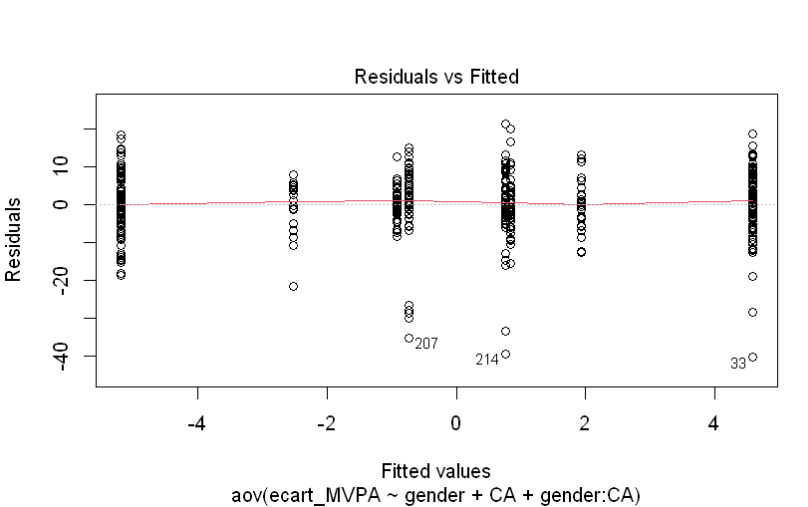
\includegraphics[width=0.8\linewidth]{variance_2.PNG}
				\caption{Graphique de diagnostic de l'homoscédasticité}
				\label{fig:variance2}
			\end{figure}
		\end{frame}
		
		\begin{frame}{Normalité des résidus du modèle}
			\begin{figure}[H]
				\centering
				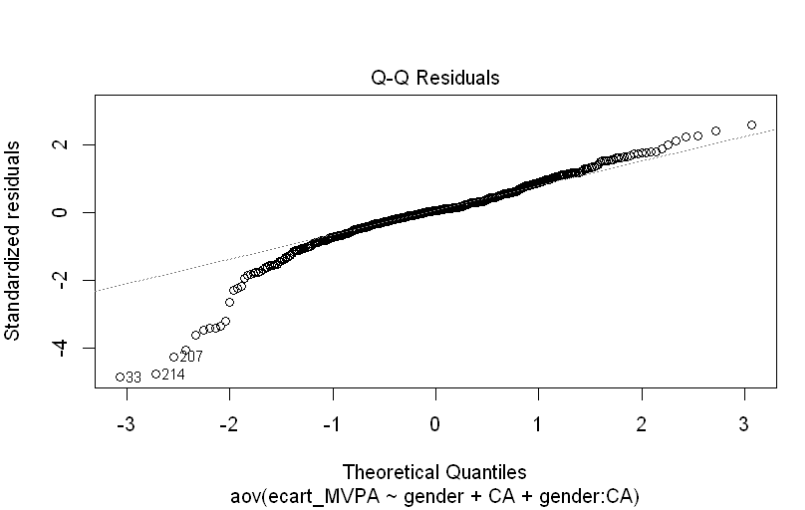
\includegraphics[width=0.8\linewidth]{Normalité_2.PNG}
				\caption{Q-Q plot}
				\label{fig:QQplot_2}
			\end{figure}
		\end{frame}
		
	\subsection{Type d'ANOVA}
	\begin{frame}{Type d'ANOVA (1/4)}
		\begin{itemize}
			\item Tester uniquement la nullité des paramètres n'est pas suffisant pour définir correctement l'hypothèse nulle ; il faut aussi considérer les hypothèses sur les autres facteurs et interactions.
			\vfill
			\pause
			\item Dans un plan équilibré, le test de significativité d'un facteur reste le même, indépendamment des hypothèses sur les autres variables.
			\vfill
			\pause
			\item Dans un plan déséquilibré, le test de significativité d'un facteur peut varier en fonction des hypothèses sur les autres facteurs et interactions.
			\vfill
			\pause
			\item Pour spécifier correctement le rôle des autres facteurs et interactions dans un plan déséquilibré, on utilise la notion de réduction.
		\end{itemize}
	\end{frame}
	
	\begin{frame}{Type d'ANOVA (2/4)}
		\textbf{Définition de la réduction}
		\begin{myblock}
			S Soit un modèle contenant les effets $(a_1,\ldots,a_l)$ des facteurs $(X_1, X_2, \ldots, X_l)$. On appelle réduction associée à l'introduction de $a_{q_1}, \ldots, a_{q_d}$ dans un modèle contenant les effets $a_{i_1}, \ldots, a_{i_m}$, notée $R(a_{q_1}, \ldots, a_{q_d}|\mu,a_{i_1}, \ldots, a_{i_m})$ la norme suivante :
			
			\begin{equation}
				R(a_{q_1}, \ldots, a_{q_d}|\mu,a_{i_1}, \ldots, a_{i_m}) = SCE_{i_1,i_2,\ldots,i_m,q_1,q_2,\ldots,q_d} - SCE_{i_1,i_2,\ldots,i_m},
			\end{equation}
			
			avec $SCE_{i_1,i_2}$ la somme des carrés expliquée par le modèle associée aux facteurs $X_{i_1}$, $X_{i_2}$.
		\end{myblock}
	\end{frame}
	
	\begin{frame}{Type d'ANOVA (3/4)}
		\textbf{Les hypothèses associés à la réduction $R(\gamma|\mu,\alpha,\beta)$ du modèle $M_1$}
		\begin{itemize}
			\item $H_0$ : Il n'y a pas de différence significative entre le modèle ne contenant pas l'effet du facteur d'interaction entre genre et CA et le modèle complet.
			\item $H_1$ : Il y a une différence significative entre le modèle ne contenant pas l'effet du facteur d'interaction entre genre et CA et le modèle complet.
		\end{itemize}
		\pause
		\textbf{ANOVA de type II}
		\begin{itemize}
			\item Évalue l'effet d'un facteur ou d'une interaction en tenant compte des autres facteurs principaux, sans dépendre de l'ordre d'introduction.
			\item L'effet d'un facteur principal ne peut pas être supprimé si une interaction est présente dans le modèle.
		\end{itemize}
	\end{frame}
	
	\begin{frame}{Type d'ANOVA (4/4)}
		\begin{table}[H]
			\centering
			\caption{Table d'analyse de la variance des réductions de type II du modèle $M_1$.}
			\resizebox{\textwidth}{!}{ % Redimensionne le tableau pour qu'il tienne dans la largeur du texte
				\begin{tabular}{|>{\centering\arraybackslash}m{2cm}|>{\centering\arraybackslash}m{3cm}|>{\centering\arraybackslash}m{2cm}|>{\centering\arraybackslash}m{3cm}|>{\centering\arraybackslash}m{5cm}|>{\centering\arraybackslash}m{5cm}|}
					\hline
					\textbf{Effet} & \textbf{Réduction type II} & \textbf{DDL} & \textbf{F} & \textbf{Loi de $F$ sous $H_0$} \\
					\hline
					$\alpha$ & $R(\alpha|\mu,\beta)$ & $I-1$ & \LARGE{$\frac{\frac{R(\alpha|\beta, \mu)}{I-1}}{\frac{\text{SCR}}{n - IJ}}$} & \LARGE{$\mathcal{F}_{I-1, n-IJ}$} \\
					\hline
					$\beta$ & $R(\beta|\mu, \alpha)$ & $J-1$ & \LARGE{$\frac{\frac{R(\beta|\mu, \alpha)}{J-1}}{\frac{\text{SCR}}{n - IJ}}$} & \LARGE{$\mathcal{F}_{J-1, n-IJ}$}  \\
					\hline
					$\gamma$ & $R(\gamma|\mu, \alpha, \beta)$ & $(I-1) \times (J-1)$ & \LARGE{$\frac{\frac{R(\gamma|\mu, \alpha, \beta)}{(I-1) \times (J-1)}}{\frac{\text{SCR}}{n - IJ}}$} & \LARGE{$\mathcal{F}_{(I-1) \times (J-1), n-IJ}$} \\
					\hline
				\end{tabular}
			}
			\label{ref:analyse_var_2}
		\end{table}
	\end{frame}
	
	\section{Résultats et discussion}
	\begin{frame}
		\tableofcontents[sections={3}]
	\end{frame}
	
	\subsection{Tableau de contingence}
	\begin{frame}{Tableau de contingence}
		\begin{table}[H]
			\centering
			\caption{Effectifs des CA par genre}
			\begin{tabular}{ccccc}
				\toprule
				& CA 1 & CA 2 & CA 3 & CA 4 \\ 
				\midrule
				F & 20 & 53 & 49 & 98 \\ 
				M & 26 & 51 & 54 & 111 \\ 
				\bottomrule
			\end{tabular}
			\label{tab:ca_gender}
		\end{table}
		
		\begin{itemize}
			\item Plan non équilibré
			\vfill
			\item ANOVA de type II
			\vfill
			\item Seuil de significativité des tests fixés à 5\%
		\end{itemize}
	\end{frame}
	
	\subsection{Test de validité du modèle complet}
	\begin{frame}{Test de validité du modèle complet}
		On teste :
		\begin{itemize}
			\item \textbf{$H_0$} : $\alpha_i = 0$ et $\beta_j = 0$ et $\gamma_{ij} = 0 \quad \forall i, j$
			\item \textbf{$H_1$} : $\alpha_i \neq 0$ ou $\beta_j \neq 0$ ou $\gamma_{ij} \neq 0 \quad \forall  i, j$
		\end{itemize}
		
		\begin{table}[H]
			\centering
			\caption{Tableau d'analyse de variance pour le modèle $M_1$}
			\begin{tabular}{ccccccc}
				\toprule
				\textbf{Res.Df} & \textbf{RSS} & & \textbf{Df} & \textbf{Sum of Sq} & \textbf{F value} & \textbf{Pr($>F$)} \\ 
				\midrule
				461 & 36916 & & & & & \\ 
				454 & 31593 & & 7 & 5323.2 & 10.928 & 8.944 $\times 10^{-13}$ \\ 
				\bottomrule
			\end{tabular}
			\label{tab:anova_results1}
		\end{table}
	\end{frame}
	
	\subsection{Test de validité de sous modèle}
	\begin{frame}{Test de validité de sous modèle}
		\begin{table}[H]
			\centering
			\caption{Effets des différents facteurs (type II) dans le modèle M1}
			\begin{tabular}{lcccc}
				\toprule
				Source & Sum Sq & Df & F value & Pr($>F$) \\ 
				\midrule
				genre & 3585.2 & 1 & 51.5200 & 2.911 $\times 10^{-12}$ \\ 
				CA & 6.4 & 3 & 0.0307 & 0.9927 \\ 
				genre:CA & 1738.0 & 3 & 8.3252 & 2.122 $\times 10^{-5}$ \\ 
				Résidus & 31592.8 & 454 & & \\ 
				\bottomrule
			\end{tabular}
			\label{tab:anova_results2}
		\end{table}
		
		\textbf{Effet de l'interaction entre genre et CA} :
		\begin{itemize}
			\item \textbf{$H_0$} : $Y_{ijk} = \mu + \alpha_i + \beta_j + \epsilon_{ijk} \quad \forall i,j,k$ 
			\item \textbf{$H_1$} : $Y_{ijk} = \mu + \alpha_i + \beta_j + \gamma_{ij} + \epsilon_{ijk} \quad \forall i,j,k$
		\end{itemize}
	\end{frame}
	
	\subsection{Test de comparaison multiple}
	\begin{frame}{Test de comparaison multiple (1/2)}
		
		Nous voulons tester les hypothèses :
		\begin{itemize}
			\item $H_0 : \theta_{i_1j} = \theta_{i_2j}$
			\item $H_1 : \theta_{i_1j} \neq \theta_{i_2j}$
		\end{itemize}
		où $\theta_{i_1j_1}$ et $\theta_{i_2j_2}$ sont les moyennes théoriques des écarts de MVPA à la moyenne de chaque classe dans chaque groupe différent et $i_1, i_2 \in \{1, 2\}$ avec $i_1 \neq i_2$ ; $j \in \{1, \ldots, 4\}$. \\
		
	\end{frame}
	
	\begin{frame}{Test de comparaison multiple (2/2)}
		\begin{table}[H]
			\centering
			\caption{Test post hoc (Tukey-Cramer)}
			\renewcommand{\arraystretch}{1.3} % Réduit légèrement l'espacement vertical pour mieux tenir sur le slide
			\resizebox{\textwidth}{!}{ % Redimensionne le tableau pour qu'il tienne dans la largeur du slide sans dépasser
				\begin{tabular}{|>{\centering\arraybackslash}p{5.5cm}|>{\centering\arraybackslash}p{2.8cm}|>{\centering\arraybackslash}p{2.8cm}|>{\centering\arraybackslash}p{2.8cm}|>{\centering\arraybackslash}p{2.8cm}|}
					\hline
					& CA1 & CA2 & CA3 & CA4 \\ 
					\hline
					Écart moyen entre filles et garçons des écarts à la moyenne de MVPA de chaque classe & -4.4548 & -1.4898 & -1.7470 & -9.7647 \\ 
					\hline
					Intervalle de confiance & -12.010 à 3.100 & -6.4730 à 3.493 & -6.759 à 3.265 & -13.286 à -6.244 \\ 
					\hline
					P-valeur & 0.6235 & 0.9850 & 0.9600 & 0.0000 \\ 
					\hline
				\end{tabular}
			}
			\label{tab:ecarts_mvpa_1}
		\end{table}
	\end{frame}
	
	\subsection{Taille d'effet}
	\begin{frame}{Taille d'effet ($\omega^2$)}
		\begin{table}[H]
			\centering
			\caption{Tailles d'effet ($\omega^2$) et intervalles de confiance à 95\% (unilatéraux)}
			\begin{tabular}{ccc}
				\toprule
				Paramètre & $\omega^2$ & 95\% CI \\
				\midrule
				Genre & 0.10 & [0.06, 1.00] \\
				CA & 0.00 & [0.00, 1.00] \\
				Genre:CA & 0.05 & [0.02, 1.00] \\
				\bottomrule
			\end{tabular}
			\label{table:effect_size_2}
		\end{table}
		\begin{itemize}
			\item L'interaction entre le genre et le CA explique 5 \% de la variance totale, ce qui représente une taille d'effet modérée.
			\vfill
			\item En EPS cette taille d'effet indique que les différences entre les filles et les garçons dans le champs 4 doivent être prise en compte.
		\end{itemize}
	\end{frame}
	
	\subsection{Limites des résultats}
	\begin{frame}{Limites des résultats}
		\begin{itemize}
			\item Le recrutement des participants parmi ceux ayant donné leur autorisation et exprimé un intérêt pourrait introduire un biais si les élèves plus motivés ou mieux équipés sont surreprésentés.
			\vfill
			\pause
			\item Les plans non équilibrés compliquent le calcul et l'interprétation des tailles d'effet, car une partie de la variabilité est perdue, rendant les tailles d'effet moins précises mais toujours indicatives de l'importance des facteurs.
			\vfill
			\pause
			\item L'examen du niveau d'engagement physique en EPS basé sur l'écart de MVPA par rapport à la moyenne de MVPA de chaque classe ne permet pas de prendre en compte les effets aléatoires liés aux collèges et aux classes appartenant àa ces collèges.
		\end{itemize}
	\end{frame}
	
	% Conclusion
	\section{Conclusion et perspective}
	\begin{frame}
		\frametitle{Conclusion}
		\begin{itemize}
			\item Les garçons sont généralement plus impliqués que les filles dans le champ 4 (activités d'opposition).
			\vfill
			\item Les autres champs (sports de performance, sports de plein air, activités artistiques) ne montrent pas de différences significatives entre les sexes.
			\vfill
			\item Analyse du niveau d'engagement en EPS basé sur le MVPA des participants avec prise en compte des effets aléatoires des collèges et des classes appartenant à ces collèges via un modèle mixte.
		\end{itemize}
	\end{frame}
	
		% Page de garde avec la barre d'en-tête vide
	{
		\setbeamertemplate{headline}{
			\leavevmode%
			\hbox{%
				\begin{beamercolorbox}[wd=.6\paperwidth,ht=2.5ex,dp=1.125ex,center]{section in head/foot}%
					% Vide pour la page de garde
				\end{beamercolorbox}%
				\begin{beamercolorbox}[wd=.4\paperwidth,ht=2.5ex,dp=1.125ex,center]{subsection in head/foot}%
					% Vide pour la page de garde
			\end{beamercolorbox}}%
			\vskip0pt%
		}
		\begin{frame}
			\centering
			\vspace{2cm}
			\Huge{\textbf{Merci pour votre attention !}}\\
			\vspace{1cm}
		\end{frame}
	}
	
	
\end{document}
